%# -*- coding: utf-8-unix -*-
%!TEX root = ..\thesis.tex

\chapter{绪论}
随着公有云和私有云架构的发展,越来越多的的网络应用和计算任务被迁移至大规模的数据中心以减少单位计算成本,数据中心的计算能力也随之不断扩展。这些数据中心由数以万计的服务器组成,其建造和运营通常花费数千万美元以上。在现代节能型数据中心的拥有成本中,购买服务器的花费占比最高,可达50-70\%\cite{barroso2013datacenter}。一直以来,摩尔定律使得新一代服务器在相同价格下都有更高的计算能力,数据中心也得以不提高花费同时持续提升规模。然而随着暗硅(dark silicon)时代的到来\cite{esmaeilzadeh2011dark}\cite{hardavellas2011toward},这样的增长将无法持续。一种解决办法是通过使用更低能耗的组件\cite{lo2014towards},如移动计算核心\cite{janapa2010web}和移动设备中使用的内存\cite{malladi2012towards}。另一种办法是通过提高服务器的利用率---显然服务器的低利用率不但使得日常运营成本偏高,也不利于收回对设备的投资。尽管低能耗组件能够降低服务器利用率时的运营成本\cite{barroso2007case},但为了考虑到服务器的巨大资本开销,研究提高数据中心的资源利用率是最有效的,也是无法避开的。

\section{服务质量(Quality-of-Service,QoS)}
% TODO ADD MULTIPLE TIME OF REQUIREMENT LIKE SLO ETC.
数据中心不同的任务面向不同的应用和用户,因此具有不同的服务质量要求。直接面向用户的应用,如社交媒体,搜索引擎,软件即服务,在线地图,网页邮箱,在线翻译,线上购物和广告等等,通常是延迟敏感型,具有很严格的服务质量要求。延迟型敏感应用通过其内部的服务基本要求(Service Level Requirements, SLAs)定义。如谷歌搜索的服务质量通过查询的延迟和每秒处理的请求个数定义;而Bing将其定义为返回结果的质量\cite{janapa2010web}\cite{kozyrakis2010server}。

数据中心还有另一类批处理任务,如文件备份,图像离线处理和视频压缩转码等等。与延迟敏感型任务相反,他们不面向用户,延迟也不敏感,因此几乎没有服务质量要求。批量分析框架可以产生大量的批处理任务,并且这些任务即使偶尔被暂停或重启,他们仍然可以产生可观的价值\cite{boutin2014apollo}\cite{carvalho2014long}\cite{curino2014reservation}\cite{delimitrou2014quasar}。

\section{资源利用率问题}
多个研究表明,数据中心的服务器平均利用率较低,介于10\%至50\%之间\cite{kaplan2008revolutionizing}\cite{vasan2010worth}\cite{reiss2012heterogeneity}\cite{barroso2013datacenter}\cite{delimitrou2014quasar}\cite{carvalho2014long},且通常不超过20\%\cite{barroso2007case}。造成资源低利用率的主要原因是存在大量的运行在严格服务质量要求下的延迟敏感型任务。这些直接面向用户的服务的运行状态和数据通常分布在多个服务器的内存和闪存之中。各个任务的用户的访问模式存在差异,因而每个任务的负载相差较大。然而,由于延迟敏感型任务普遍巨大的数据量和高昂的移动代价,这些服务难以被集中在少量服务器中,因而难以优化他们的计算资源利用率。

数据中心的服务器通常区有2-4个处理器插口,每个插口上有4-10个核心。核心之间共享一些资源,如末级高速缓存(Last Level Cache,LLC),动态随机存储器,输入输出通道,网络连接。这种共享使得各个核心之间产生难以预测的干扰,而即使轻微干扰便可能导致延迟敏感型任务违反服务质量要求\cite{janapa2010web}\cite{nesbit2006fair}\cite{meisner2011power}。为了避免违反服务质量要求,通常禁止在运行延迟敏感任务的服务器上执行其他任务。这样过度的限制使得延迟敏感型任务独占服务器,部分核心空闲,系统的资源利用率降低。例如,Google用以运行网页搜索服务的服务器24小时内的平均空闲率为30\%\cite{lo2014towards}。对延迟敏感型任务的过度保护代价高昂,同时也是不必要的。制定合理的混合执行策略可以有效提高服务器资源利用率\cite{delimitrou2013paragon}\cite{mars2011bubble}\cite{marshall2011improving}。

\section{混合执行}
数据中心的应用通常由一至数百个任务组成,每个任务有其单独的二进制程序,相关数据,以及一个声明其所需求资源的配置文件\cite{mishra2010towards}。配置文件一般包括其需要的核心数量,内存大小,硬盘空间和是否需要禁止与其他任务混合执行。一个任务调度的简化版本可见\ref{fig:schedule}。集群级别的任务调度器收到任务时,通过类似装箱问题的算法将各个任务分配至集群内的服务器上运行\cite{mishra2010towards}。当任务到达指定服务器上时,服务器级别的资源调度器将会控制任务的执行\cite{banga1999resource}。任务的资源需求通常由管理员精心配置以满足其服务质量要求。禁用混合执行的延迟敏感型任务不可避免的会占用更多的服务器资源,进而导致资源利用率下降。延迟敏感型任务严格的服务质量要求,使得我们似乎必须在延迟敏感型任务的服务质量和资源利用率之间做出选择。事实是,延迟敏感型任务独占服务器的策略通常是不必要的--尽管其他任务的执行会降低延迟敏感型任务的服务性能,但并非一定导致其违反服务质量要求。图\ref{fig:colocate}(a)表示一个来自谷歌搜索的关键组件的性能(以响应延迟的倒数表示)随同一处理器上混合执行的其他任务的影响的变化,可以看出当来自混合执行任务的干扰较低时,延迟敏感型任务的性能依然可满足服务质量要求\cite{mars2011bubble}。图\ref{fig:colocate}(b)显示了该搜索组件与多种具体任务混合执行时产生的性能下降,可以看到该搜索组件与地图等任务混合执行时仍能达到规定的服务质量;而其与广告等任务混合执行时,将产生显著的性能下降,且违反服务质量要求。

\begin{figure}
  \centering
  \begin{subfigure}{0.4\textwidth}
    \centering
    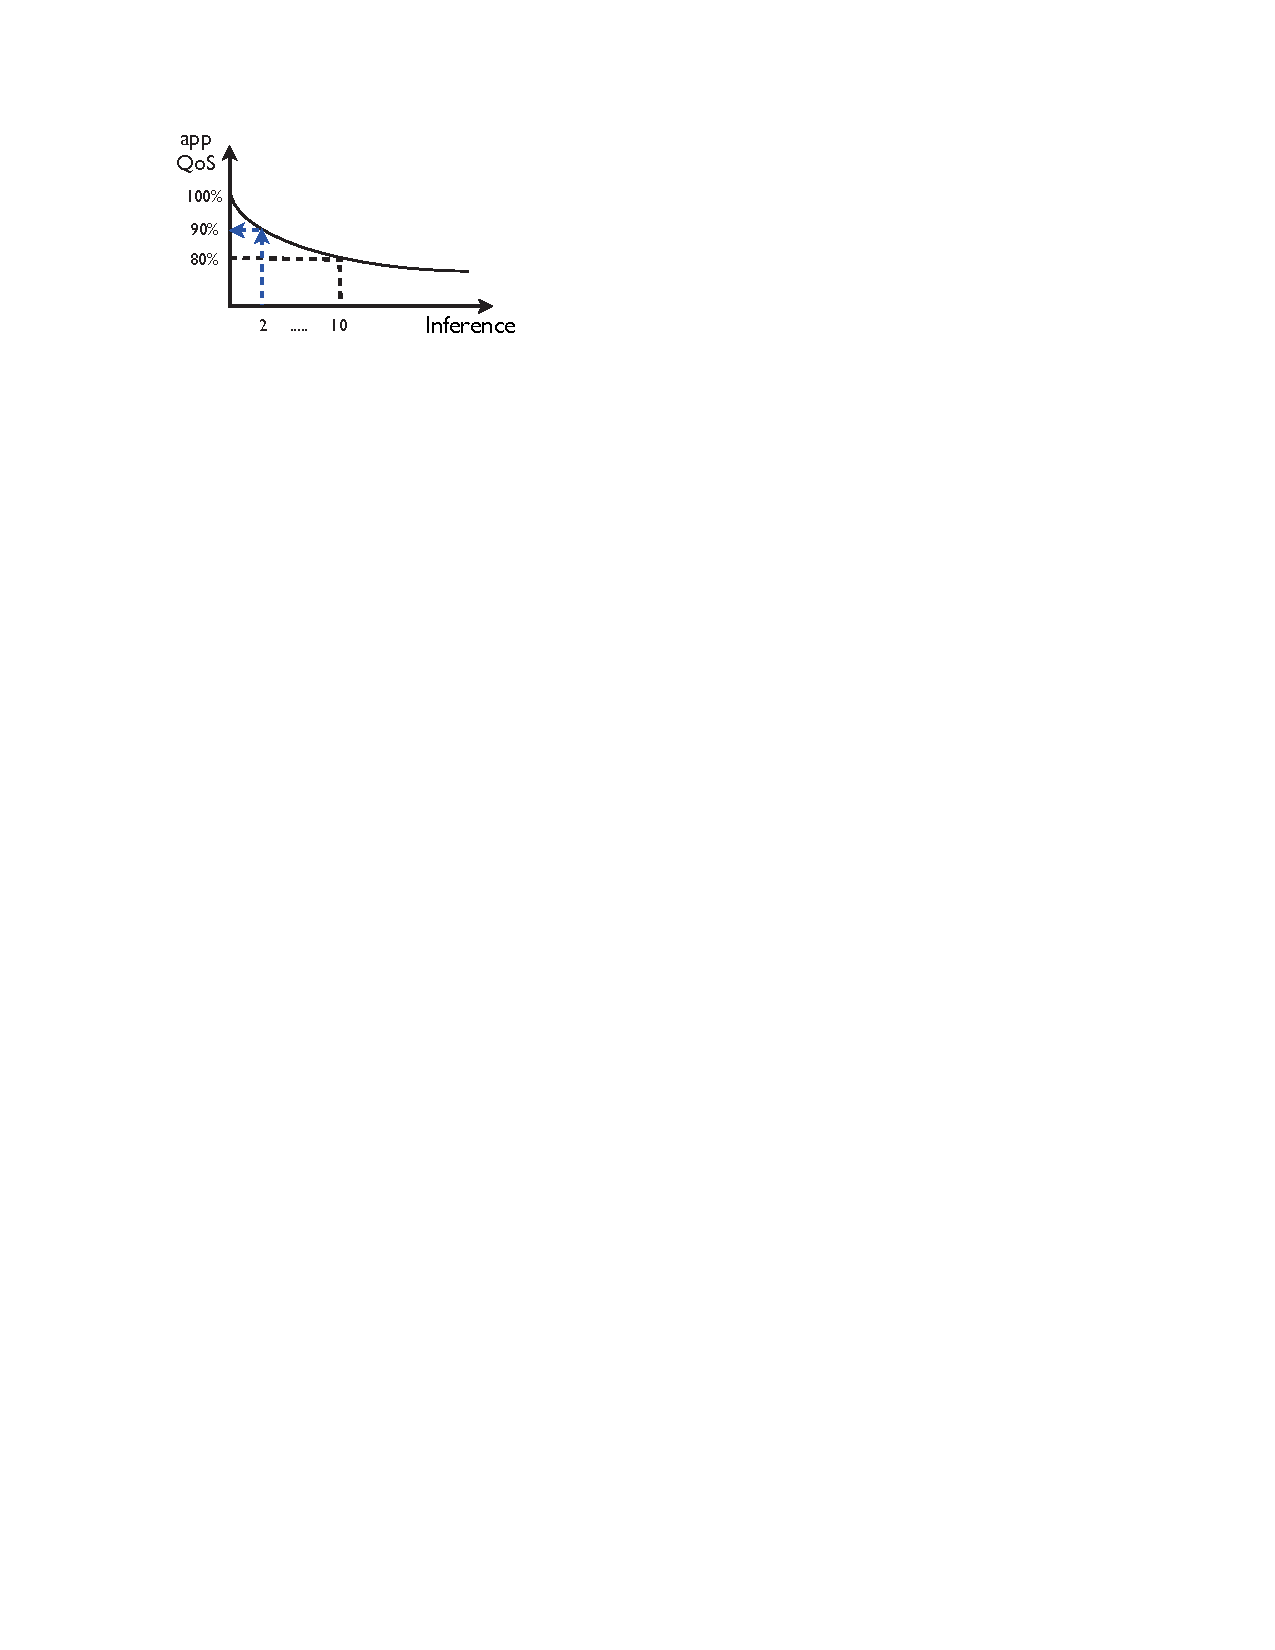
\includegraphics[height=4cm]{res_mgmt/qos_pressure.pdf}
    \caption{延迟敏感型任务服务质量随干扰强度的变化}
  \end{subfigure}
  \hspace{1em}
  \begin{subfigure}{0.55\textwidth}
    \centering
    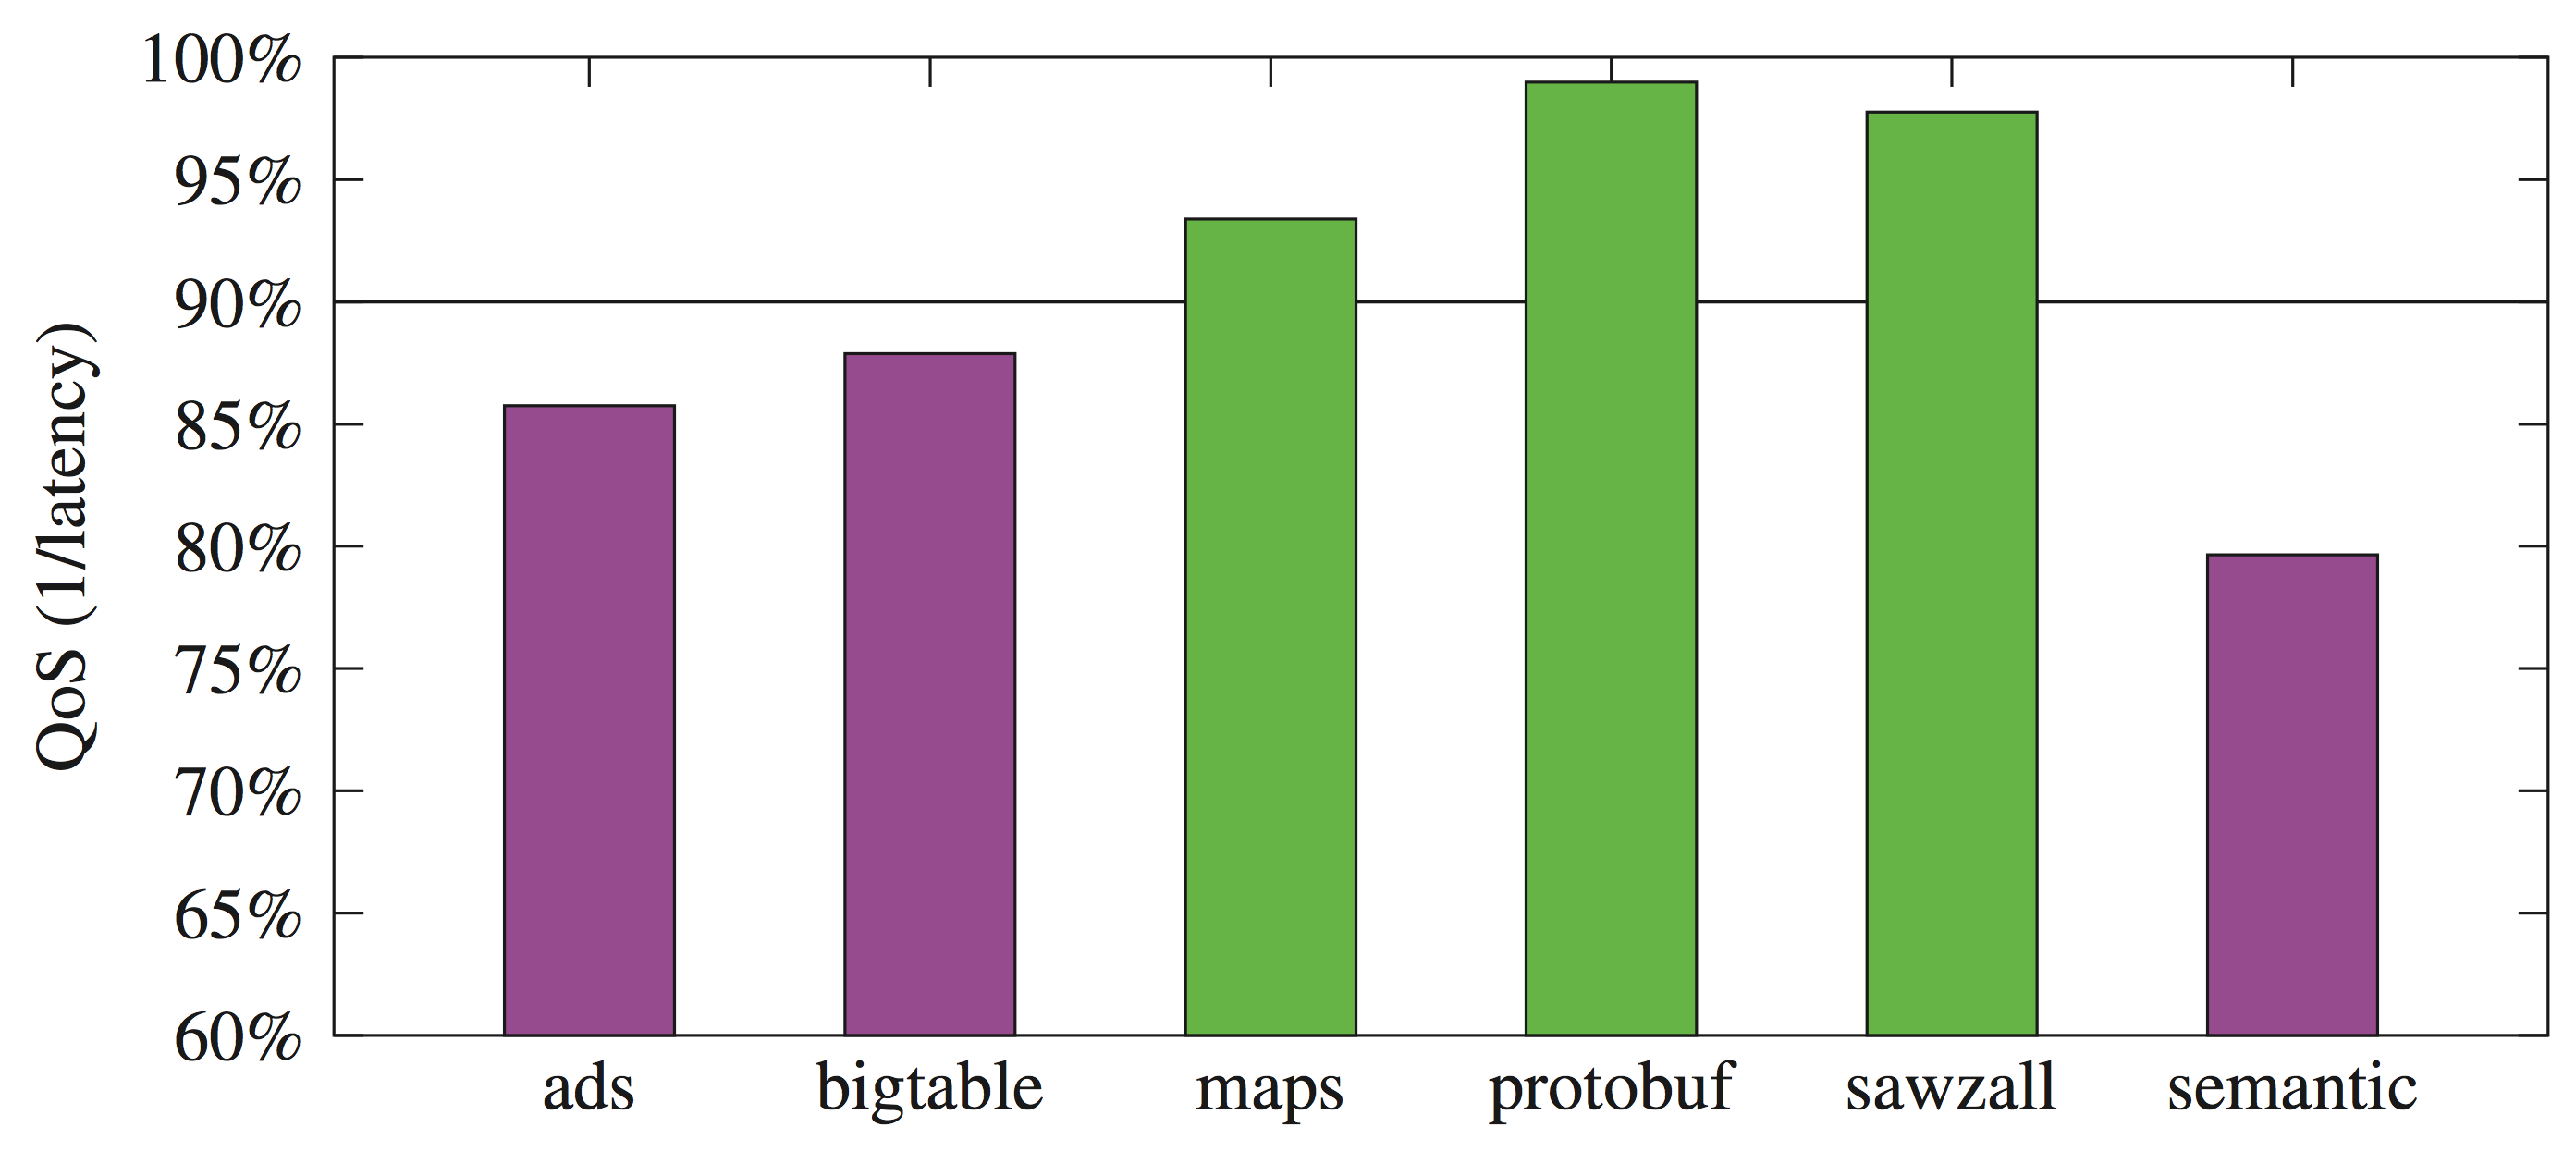
\includegraphics[height=4cm]{res_mgmt/colocate.png}
    \caption{搜索任务在混合执行时的服务质量下架}
  \end{subfigure}
  \captionof{figure}{混合执行与服务质量下降}
  \label{fig:colocate}
\end{figure}

合理地混合执行延迟敏感型任务与批处理任务,使批处理任务有机会利用延迟敏感型任务没有足够利用的资源,有利于提高整体资源利用率。混合执行的一个主要挑战在于难以确定批处理任务对共享资源产生影响,其对延迟敏感型任务的干扰更是难以预测。正因为如此,关于混合执行的研究通常关注吞吐量的任务和批处理任务的混合\cite{cook2013hardware}\cite{nathuji2010q}。

\begin{figure}
  \centering
  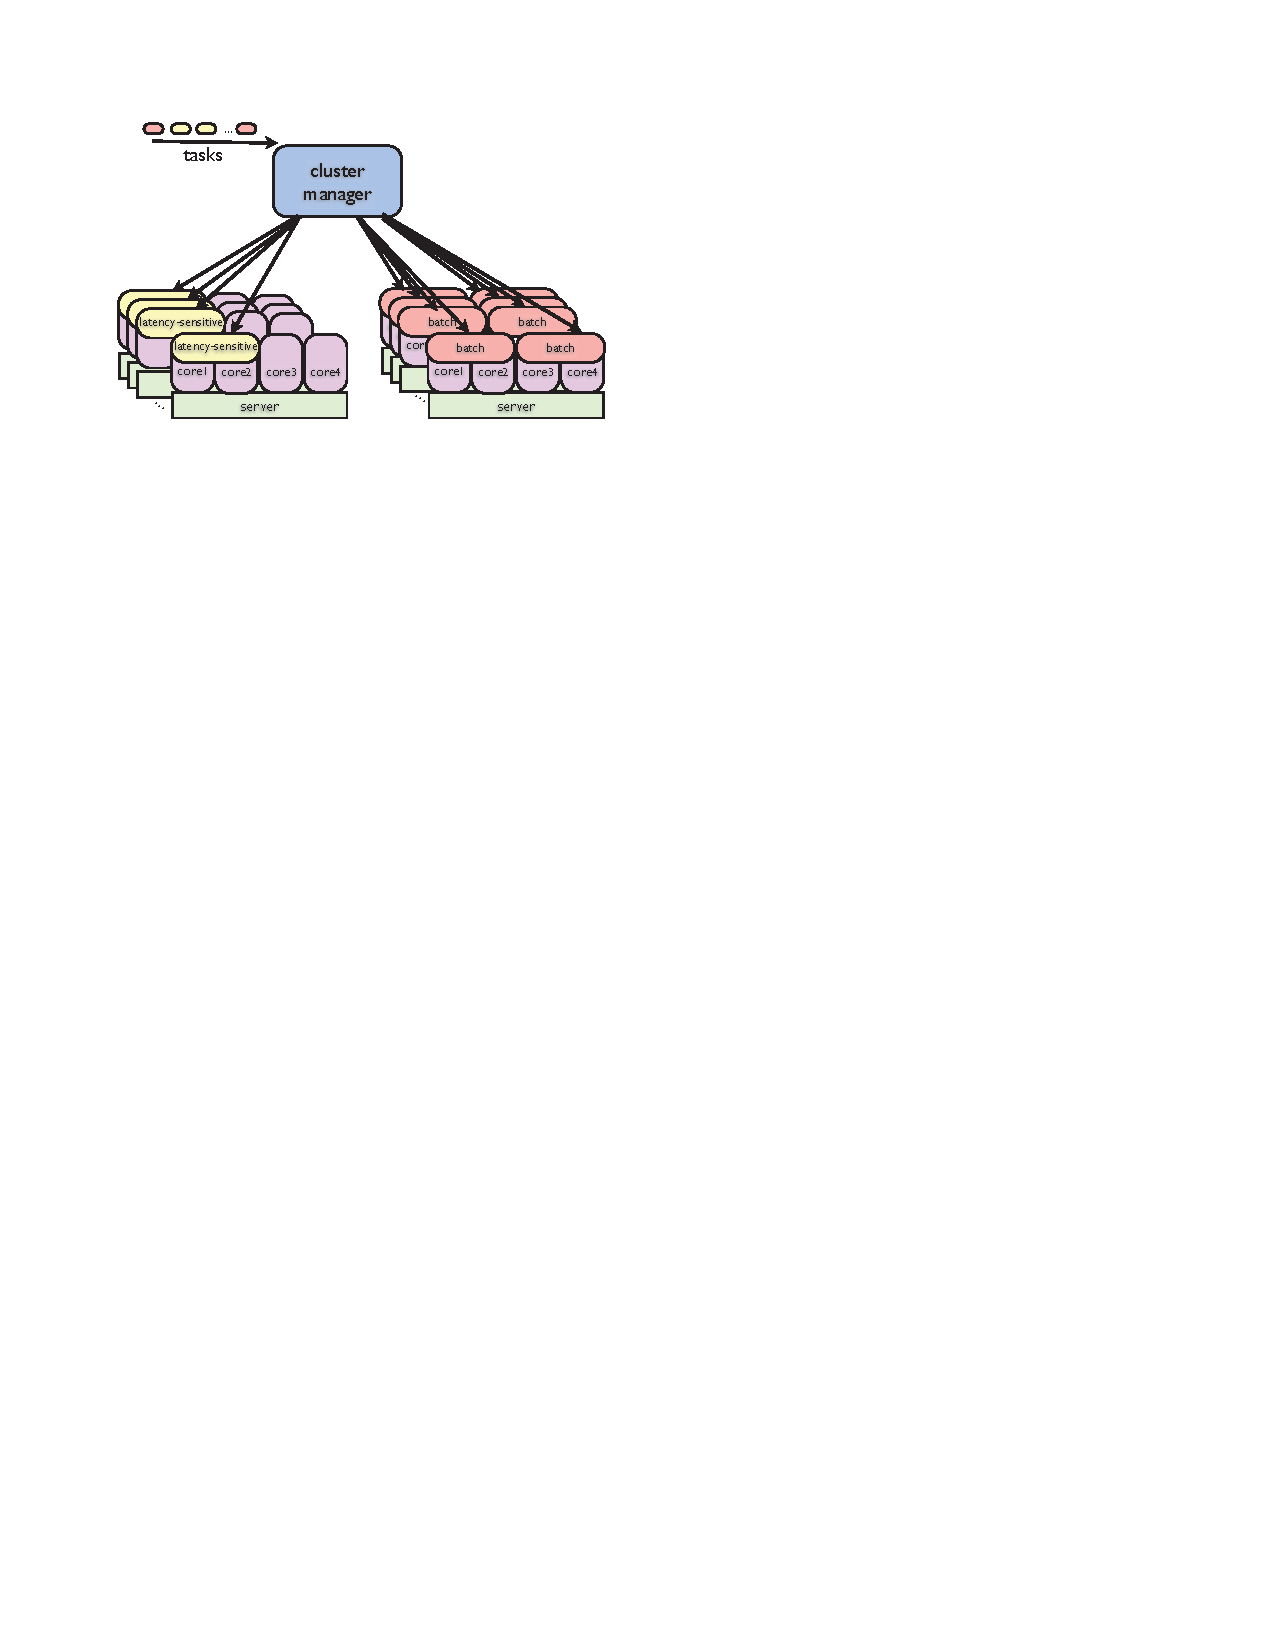
\includegraphics[width=0.65\linewidth]{res_mgmt/schedule.pdf}
  \captionof{figure}{数据中心集群级任务调度}
  \label{fig:schedule}
\end{figure}

\section{气泡测试(Bubble-Up)}
确定延迟敏感型任务和批处理任务的混合执行策略是困难的。批处理任务对延迟敏感型任务产生的性能影响很难准确预测,这导致了大部分延迟敏感型应用直接禁止混合执行。若无法对其影响准确预测,指定混合执行策略的唯一途径则只能是一一测试不同的任务混合执行的效果。对$\mathrm{N}$个任务进行测试,则需要$\mathrm{O(N^2)}$次实验。对于数据中心成百上千的应用程序和其频繁的升级更新,这种蛮力测试的代价显然是无法接受的。

Mars等人提出了气泡测试的方法来预测混合执行任务之间相互的性能影响\cite{mars2012increasing}。气泡测试将预测混合执行的任务之间的相互干扰分为两部分,一部分是任务受共享内存系统压力导致的性能下降,另一部分为其本身对共享内存系统造成的压力,如图\ref{fig:bubble}所示\cite{mars2012increasing}。第一步,通过精心设计的气泡(测试任务)来测试目标任务对内存子系统压力的的敏感程度;第二步通过测试目标任务对气泡造成的影响来预测其系统造成的压力。当混合执行导致的性能下降可以低廉代价准确预测时,即可通过类似装箱的算法找到充分利用服务器资源而不至于使延迟敏感型任务违反服务质量代价的混合策略。


气泡测试可以准确的预测延迟敏感型任务在不同程度资源竞争条件的性能下降,并以此生成任务混合策略。任务的混合执行使得服务器的资源利用率提高,然而在生成混合策略时必须考虑到延迟敏感型任务最大的资源需求。延迟敏感型任务通常面向用户,其负载虽具有固定的访问模式,但具有无法预测的访问高峰。这样的差异意味着延迟敏感型任务在相当时间内并没有全部利用预留的资源。任何静态的混合执行策略要么过于保守——导致资源利用率不足;要么过于乐观——导致延迟敏感型任务违反其服务质量要求\cite{lo2015heracles}。

解决此问题的一个办法是使用动态的混合执行策略,在应用程序高峰与低谷时执行不同的混合策略。当延迟敏感型任务处于低负载时,将其与较多占用共享资源的批处理任务混合执行;当延迟敏感型任务的负载上升时,将高共享资源占用的批处理任务迁移至其他服务器,并调度较低共享资源占用的批处理任务至当前服务器。延迟敏感型任务负载的高峰通常难以预测,且数据中心任务较大的运行时数据意味着高昂服务器间迁移任务的代价。同时,迁移任务所需的计算能力、缓存占用、网络带宽使用也会对资源敏感型任务的服务质量造成压力。另外,动态混合策略还可能存在已进行计算的进度难以保存的问题。因此通过动态的混合执行策略来提高服务器资源利用率并不实际。

另一个解决静态混合执行策略的办法则是按延迟敏感型处在低强度负载时的性能需求来确定能与之并行执行的批处理任务。这样的批处理任务具有更高的资源需求,可以在延迟敏感型任务低负载时充分利用服务器资源;在延迟敏感型任务高强度负载时并需要的大量的服务器资源时,通过资源隔离的机制保证其性能。
\begin{figure}[!t]
  \centering
    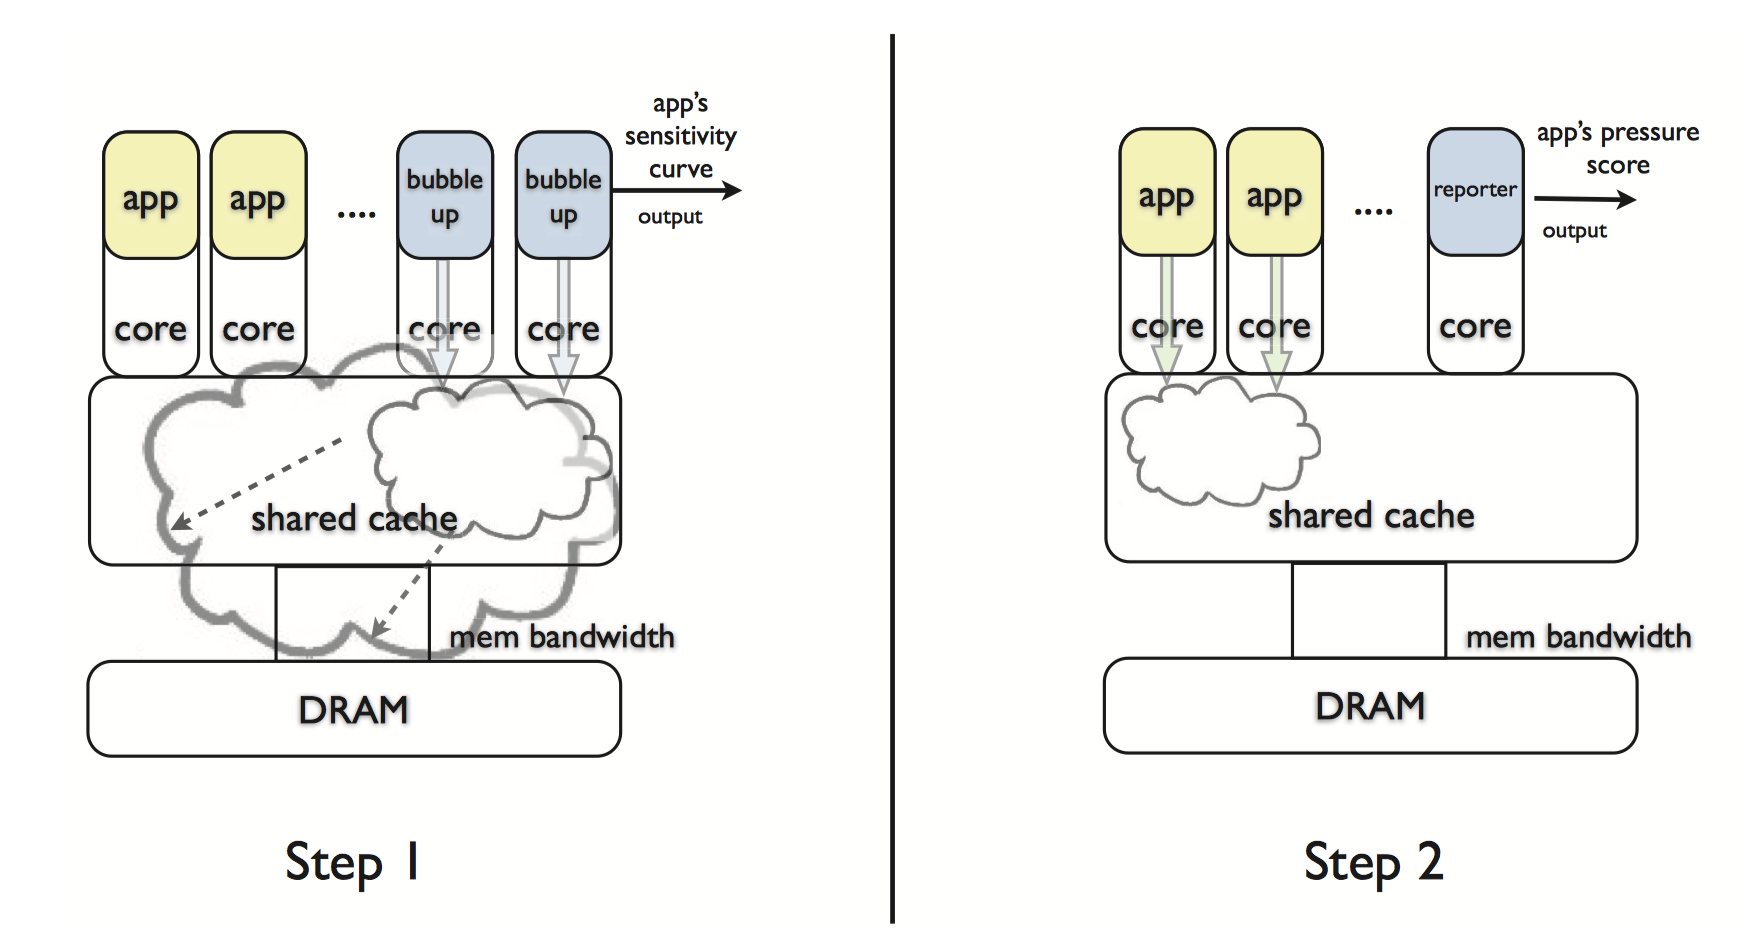
\includegraphics[width=0.95\linewidth]{res_mgmt/bubble.png}
    \captionof{figure}{气泡测试方法}
    \label{fig:bubble}    
\end{figure}
\section{资源隔离技术}
敏感型任务与批处理任务混合执行时,共享资源的相互干扰使得我们难以控制批处理任务对延迟敏感型任务的影响,进而难以保证不违反延迟敏感型任务的服务质量要求。一个典型的混合执行的任务之间在共享资源上相互干扰的例子是吵闹的邻居问题\cite{verboven2013black},即混合执行的任务在某一个或多个共享资源上进行了过多的占用。图\ref{fig:neigbor}中,蓝色线表示延迟敏感型任务的性能,红线表示批处理任务的性能。可以看到,当批处理任务不受限制地占用共享资源时,延迟敏感型任务的性能将因此出现显著下降。批处理任务不公平和不受控制的占用共享资源可能来自多个方面。

\begin{itemize}
  \item 批处理任务具有很高的并行性,因此产生了大量的进程或线程并行执行并由此抢占大量的处理器运行时间;
  \item 批处理任务使用大规模数据集且频繁读写,由此占用大部分的共享缓存和动态随机存储访问带宽,使得批处理任务的缓存命中率降低和动态随机存储器的访问延迟上升;
  \item 延迟敏感型任务使用的TCP协议在检测到网络阻塞时会主动降低带宽占用,当批处理任务使用UDP等没有流量控制的协议,批处理任务的流量不受限制的挤压延迟敏感型任务的网络带宽。
\end{itemize}

\begin{figure}
  \centering
    \centering
    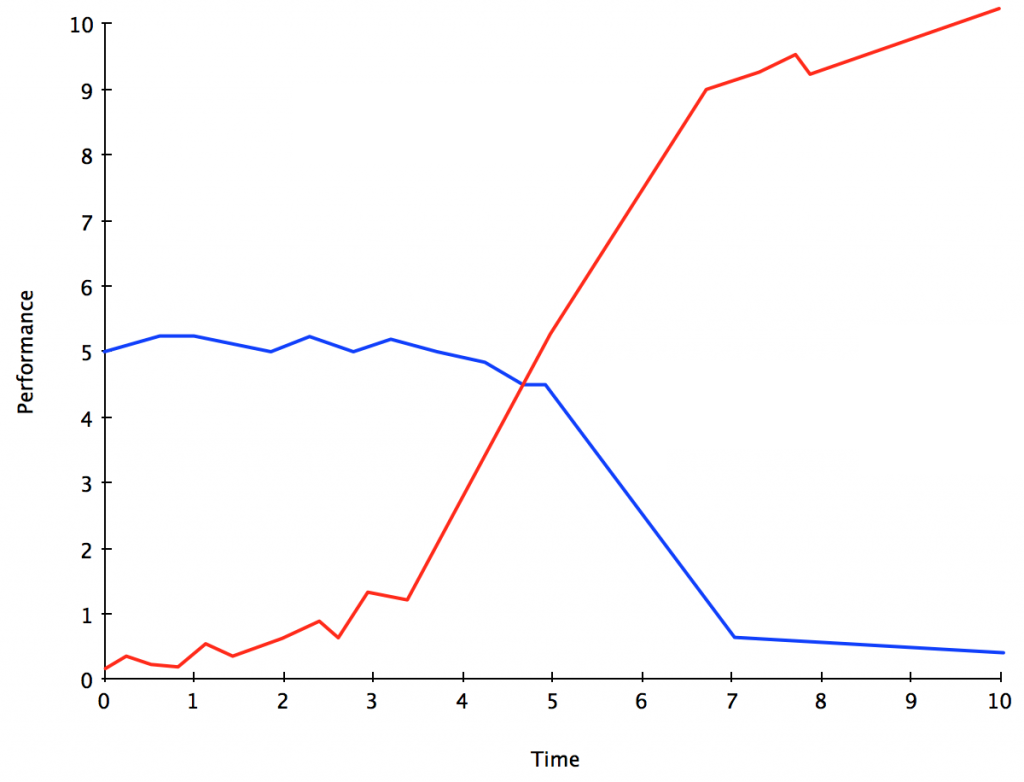
\includegraphics[width=0.6\linewidth]{res_mgmt/neighbor.png}
    \captionof{figure}{吵闹的邻居}
    \label{fig:neigbor}  
\end{figure}


混合执行任务在共享资源上相互干扰的问题,使得延迟敏感型任务的性能下降和出现不稳定,保证其服务质量成为难题。新出现的一些资源隔离技术可以让我们在单个服务器中动态分配共享资源,使得我们能够通过同时协调多种资源的分配,在采用更激进的混合执行策略的同时,改善混合执行对延迟敏感型任务服务质量的影响。

\subsection{计算核心}
核心的共享对延迟敏感型任务的服务质量影响巨大\cite{lo2015heracles},英特尔处理器的超线程技术使得问题更加复杂化。我们通常不允许延迟敏感型任务和批处理任务共享一个逻辑核心(一个超线程),因为在共享逻辑核心时,操作系统内核的调度会增加即使毫秒的延迟\cite{leverich2014reconciling}。另外当同属一个物理核心的两个超线程同时执行延迟敏感型任务和批处理任务,他们将共享指令带宽,一/二级高速缓存和页表缓存。实验表明,当延迟敏感型任务与其他计算密集或访存密集的任务共享同一物理核心时(运行在不同逻辑内核上),敏感型任务的服务质量会出现显著下降\cite{lo2015heracles}。

通过Linux的\textit{cgroup}框架\cite{menage2008cgroups}我们可以将延迟敏感型任务和批处理任务隔离在不同的逻辑核心子集上。随着服务器的逻辑计算核心数目增多,这样的资源调度也更为细粒度。计算核心的分配可以动态调节,调节的速度取决于Linux内核可以在多快时间内将任务从一个核心迁移到另外一个核心,这通常在几十毫秒左右。

\subsection{末级高速缓存}
同一处理器接口上的核心共享末级高速缓存。多个研究表明共享末级高速缓存中不受控制的干扰会严重影响混合执行任务的性能\cite{delimitrou2014quasar}\cite{govindan2011cuanta}\cite{leverich2014reconciling}\cite{mars2012increasing}\cite{sanchez2011vantage}。混合执行任务在末级高速缓存上不受控制的干扰是一个典型的吵闹的邻居问题,如图\ref{fig:cache_diagram}。图\ref{fig:cache_diagram}(a)中,批处理任务有高频率的数据读取需求,在没有末级高速缓存隔离时,批处理任务占用了大量的缓存容量。对延迟敏感型任务来说,尽管通过计算核心隔离技术获得了较大的计算核心资源,其实际可用的缓存大小却严重低于需求,引起缓存命中率的将下降,整体性能也将下降。当延迟敏感型任务处于高负载状态时,轻微的相互干扰会引起巨大的延迟\cite{kasture2014ubik},因此末级高速缓存的干扰可能造成延迟敏感型任务违反服务质量要求。

\begin{figure}
  \centering
  \begin{subfigure}{0.4\textwidth}
    \centering
    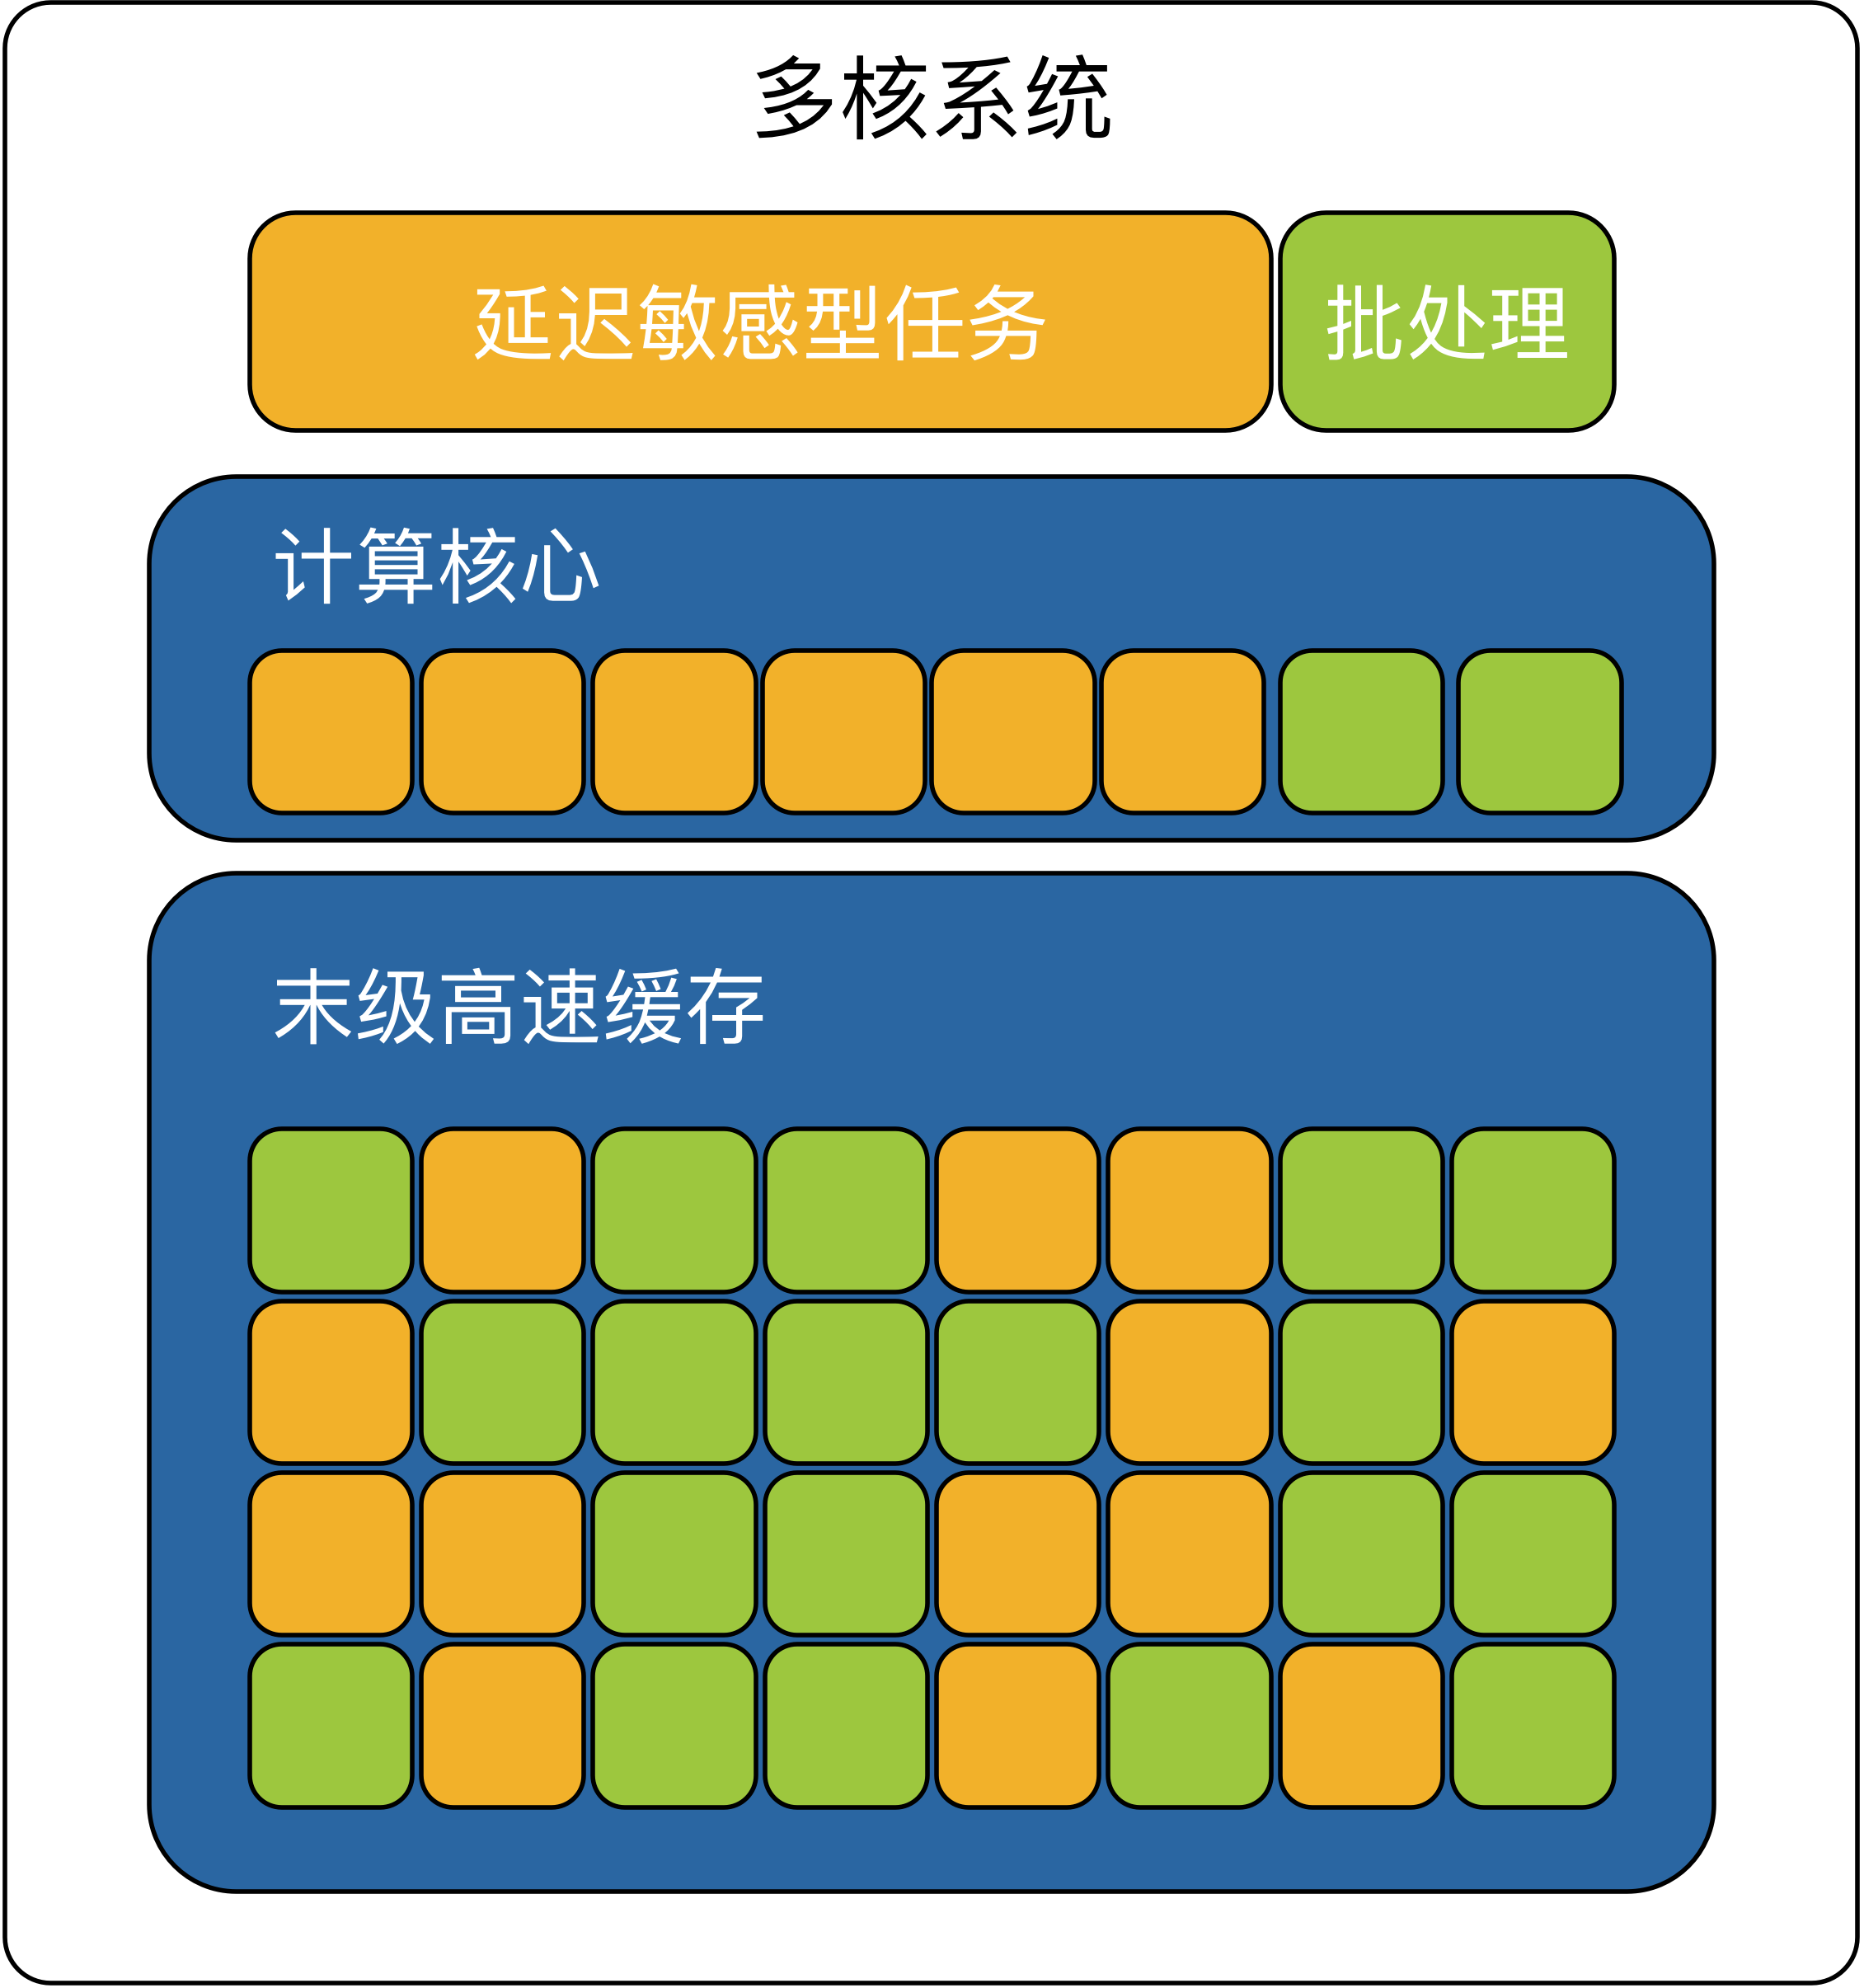
\includegraphics[height=7cm]{res_mgmt/cache_diagram_a.png}
    \caption{批处理任务过多占用缓存}
  \end{subfigure}
  \hspace{3em}
  \begin{subfigure}{0.4\textwidth}
    \centering
    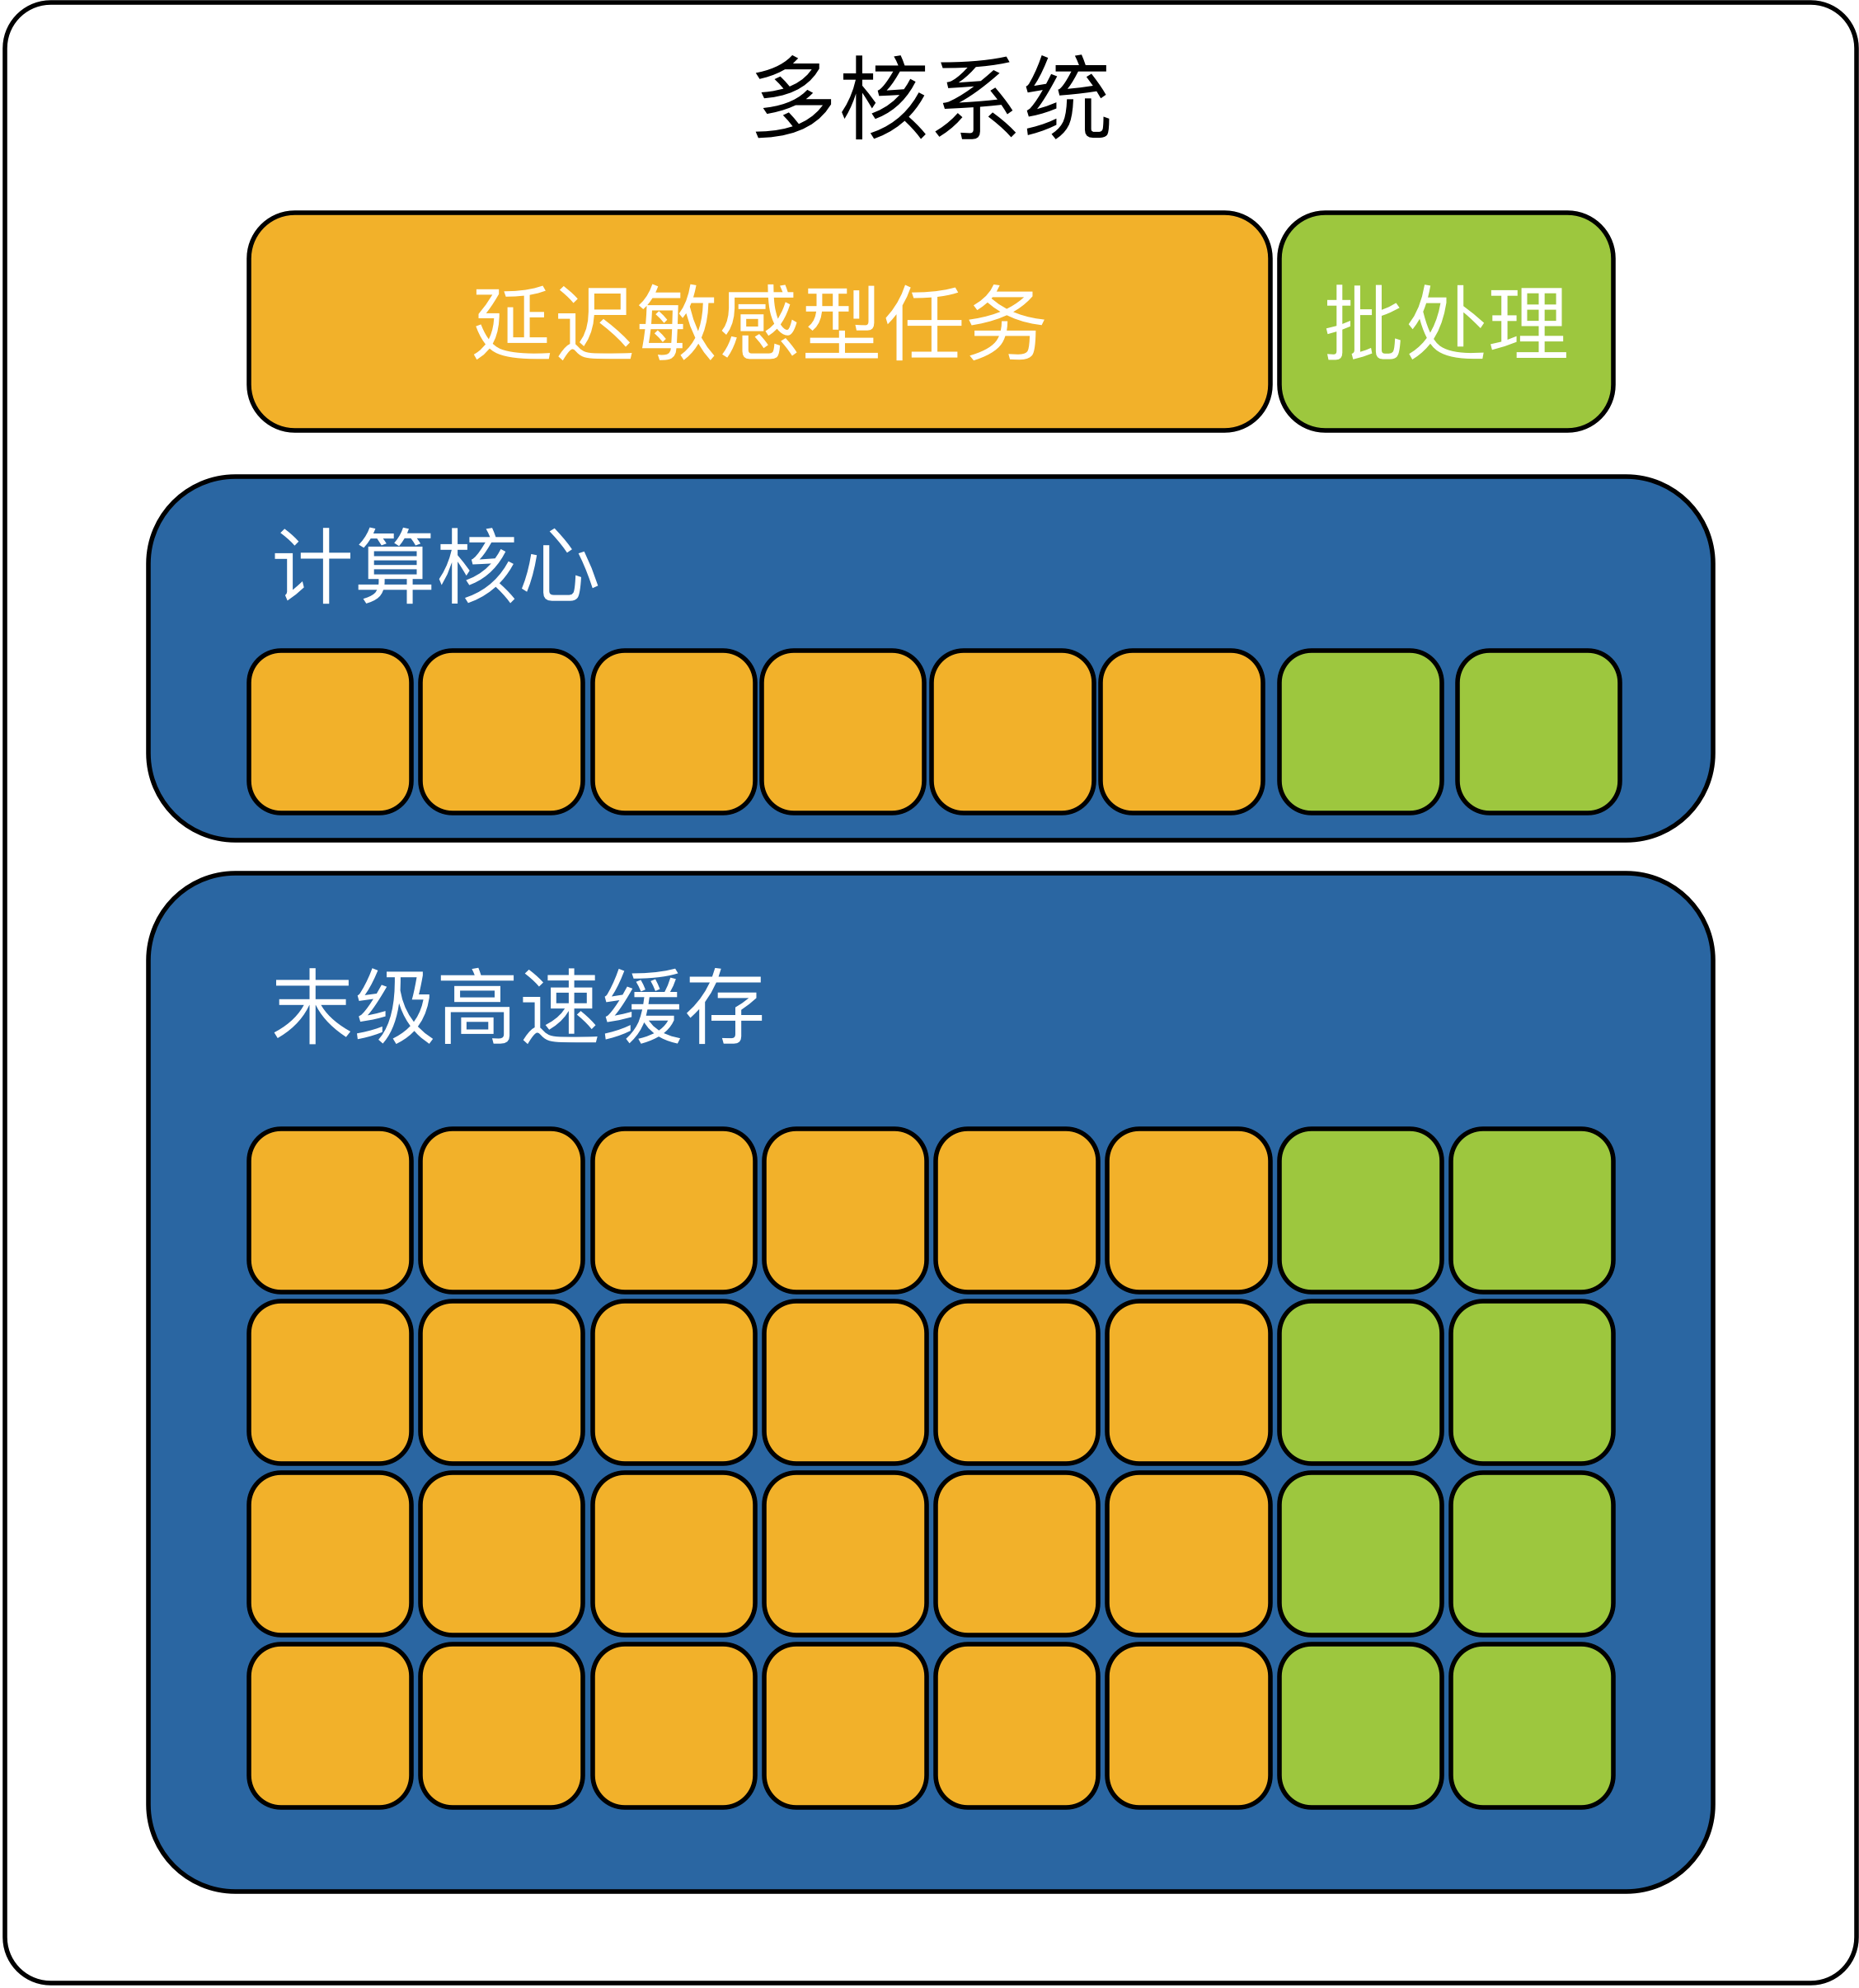
\includegraphics[height=7cm]{res_mgmt/cache_diagram_b.png}
    \caption{缓存分配技术隔离缓存使用}
  \end{subfigure}
  \captionof{figure}{末级高速缓存上的相互干扰}
  \label{fig:cache_diagram}
\end{figure}


% Thread ID and cache line
混合执行任务抢占末级高速缓存的问题一直无法有效解决,直到近期硬件支持的资源管理技术的出现。英特尔自Xeon E3引入的缓存分配技术(Cache Allocation Technology, CAT)基于硬件实现了末级高速缓存按路分配管理\cite{guide2011intel}。缓存分配技术将末级缓存按组关联路数划分成更小的缓存子集。当核心被分配给某一缓存子集后,可以在缓存任何位置命中,但新读取的数据只能写入其被分配的子集之中。通过缓存分配我们可以为延迟敏感型任务和批处理任务分配不相重叠的末级高速缓存以限制批处理任务在末级缓存处对延迟敏感型任务产生的压力。即使是将批处理任务与只关注吞吐量的任务混合执行时,通过硬件或软件技术动态分配末级高速缓存也是被普遍偏好的做法\cite{cook2013hardware}\cite{iyer2007qos}\cite{qureshi2006utility}\cite{lin2008gaining}\cite{nathuji2010q}。改变缓存分配可以通过写特定寄存器(Model Specific Register, MSR)动态实现并在在数毫秒内生效,其粒度通常在末级高速缓存大小的5\%左右\cite{herdrich2016cache}。Linux内核自4.10起通过虚拟文件系统resctl也实现了对缓存分配技术的支持。

通过缓存分配技术,我们可以实现混合执行任务间末级高速缓存资源的隔离。图\ref{fig:cache_diagram}(b)中,通过缓存分配技术,延迟敏感型任务被分配与之计算核心资源成比例的末级高速缓存容量,避免了来自批处理任务的干扰以获得稳定的服务性能。图\ref{fig:cat_perf}显示压缩任务Bzip2与各种任务混合执行时,缓存分配技术(CAT)的使用对其性能的稳定作用\cite{herdrich2016cache}。可以看到Bzip2对来自部分产生较大缓存压力的应用的干扰敏感;同时还能看到,合理的隔离不同任务对末级高速缓存的共享(实验中为Bzip2分配50\%的末级高速缓存),使得Bzip2任务在混合执行条件下基本保持与单独执行时一致的性能。

\begin{figure}
  \centering
  % \begin{minipage}[b]{0.6\textwidth}
    \centering
    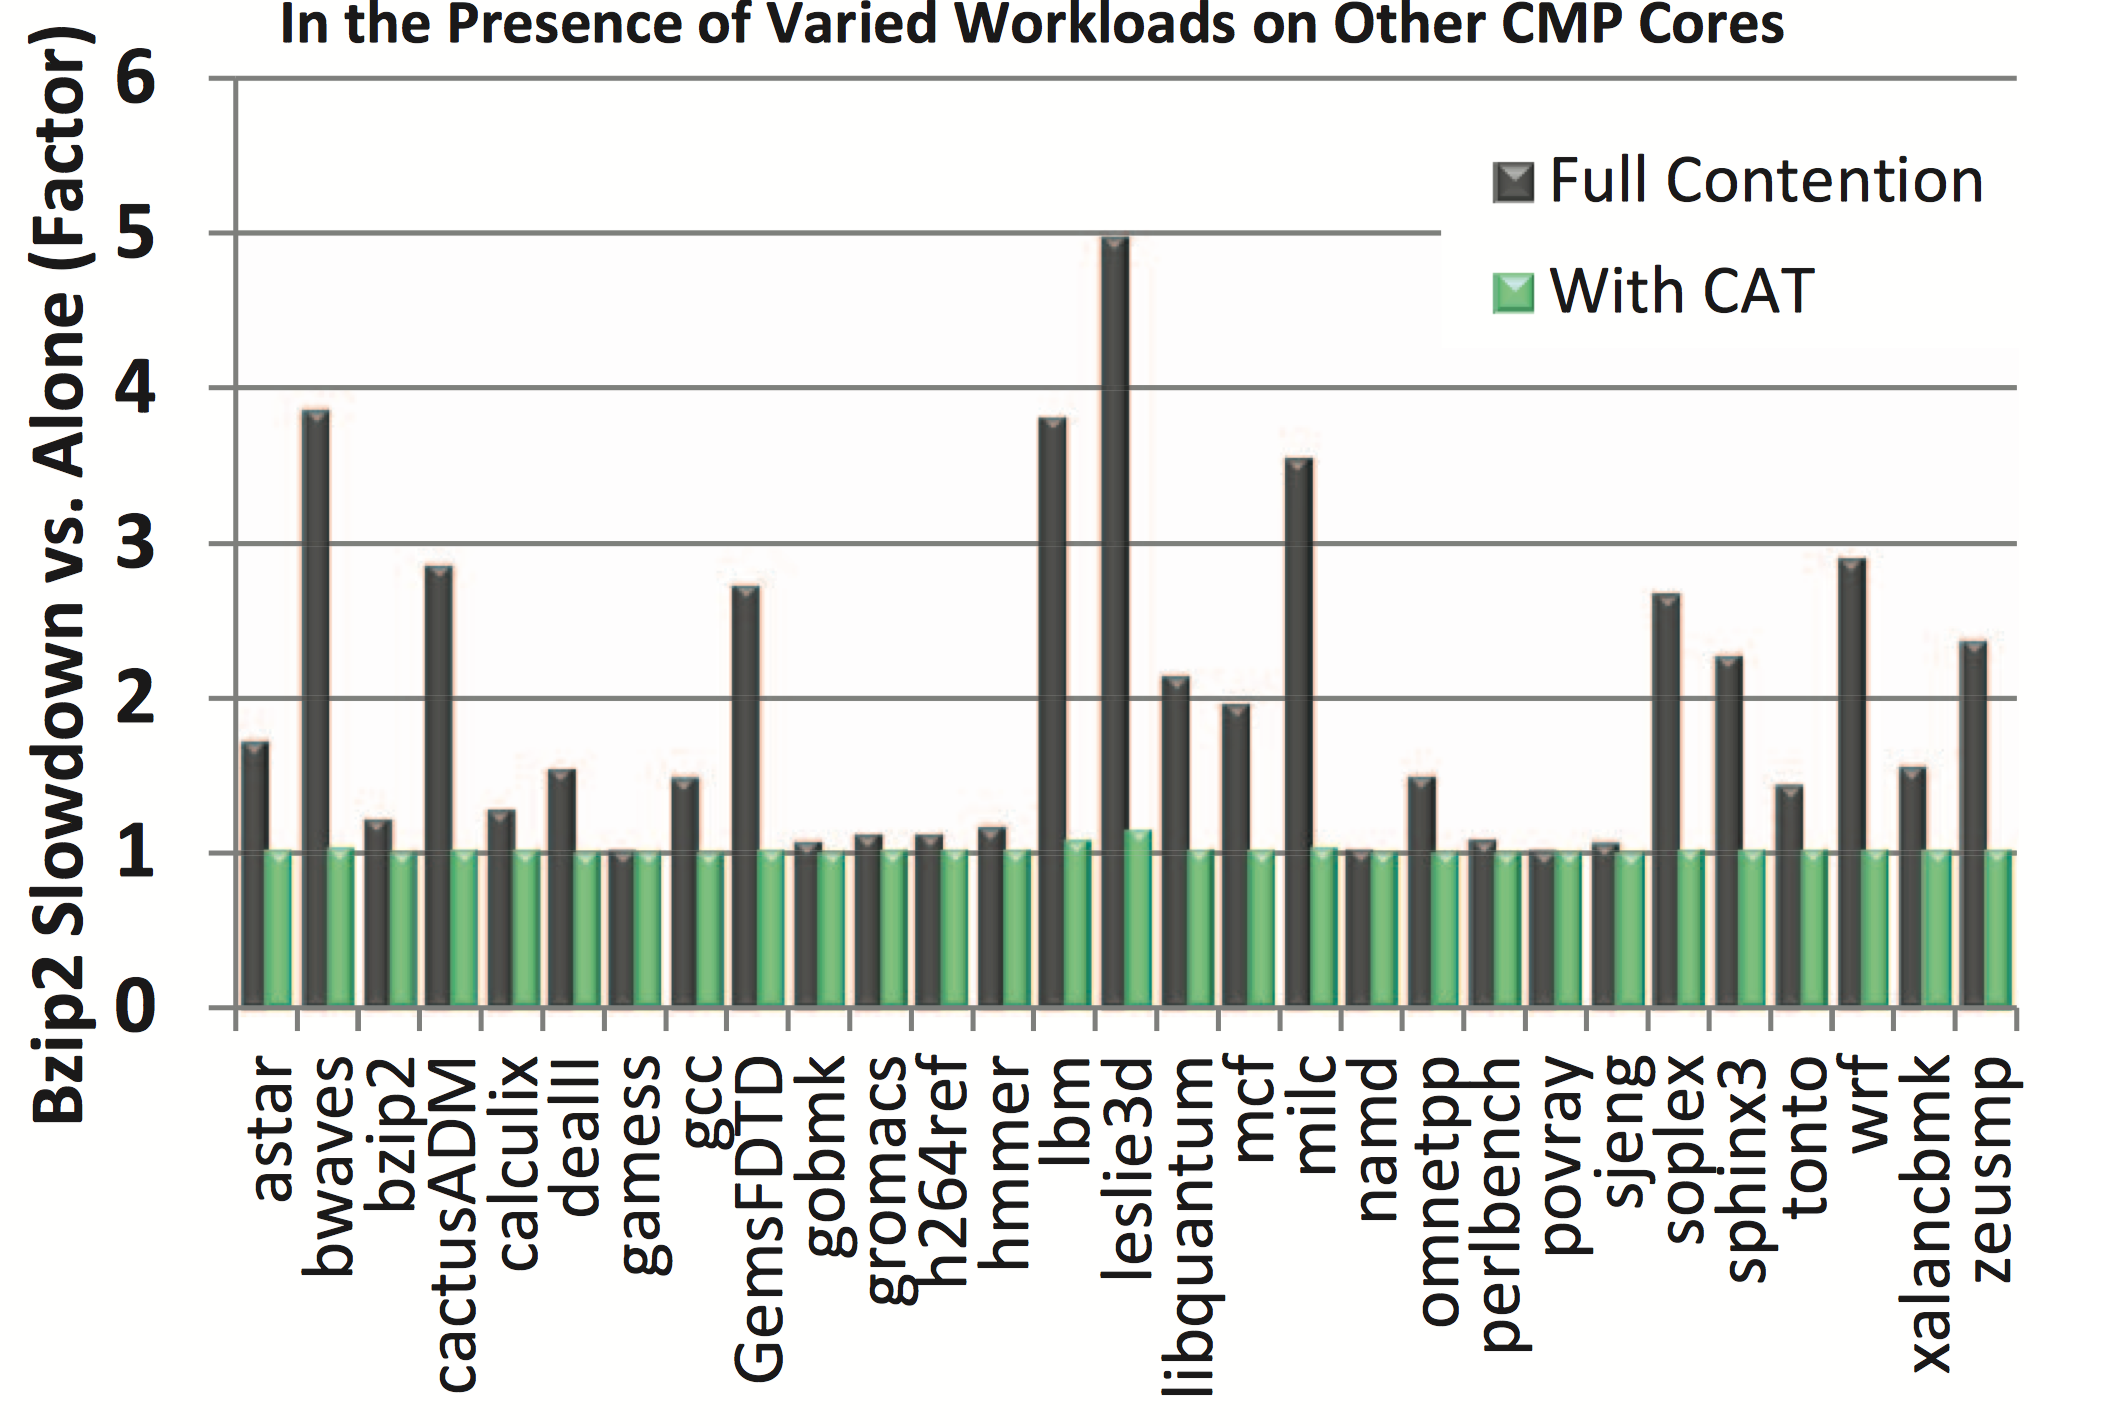
\includegraphics[width=1\linewidth]{rl/cat_perf.png}
    \captionof{figure}{Bzip2混合执行时的性能下降}
    \label{fig:cat_perf}
  % \end{minipage}     
\end{figure}

\subsection{动态随机存储器访问带宽}
数据中心的大部分的任务,无论是延迟敏感任务或批处理任务,都运行在较大的数据集之上,无法载入片上高速缓存。因此,这些任务在执行时都将占用动态随机存储器的访问带宽,且对混合执行的任务访问动态随机存储产生干扰。当批处理任务的末级高速缓存使用受限后,其末级缓存的命中率也会降低,导致其对动态随机存储的访问增加并占用更多的访存带宽。批处理任务占用更高的动态随机存储器访问带宽意味着当延迟敏感型应用内存读写的代价升高,进而可能导致其违反服务质量要求。因此动态控制批处理任务的动态随机存储器带宽占用有利于减小资源敏感型任务读写内存性能受到的干扰。

已有大量的研究致力于解决混合执行任务的动态随机存储访问上的相互干扰\cite{iyer2007qos}\cite{jeong2012qos}\cite{muralidhara2011reducing}\cite{nesbit2006fair}。最新的英特尔处理器引入了内存带宽分配(Memory Bandwidth Allocation, MBA)技术和内存带宽监控(Memory Bandwidth Monitoring)技术\cite{iyer2007qos}\cite{guide2011intel}。内存分配技术仅在部分新处理器可用,大部分处理器硬件仅支持内存带宽监控\cite{guide2011intel}。幸运的是,基于硬件且粒度为单个核心的内存带宽监控配合动态的计算核心分配技术,我们能够粗粒度的调控批处理任务对动态随机存储器访问带宽\cite{lo2015heracles}。当监测到批处理任务过多占用内存访问带宽而延迟敏感型任务受限与此时,可以通过减少为其分配的计算核心以降低其带宽占用。尽管如此,缺少硬件支持的对动态随机存取器访问带宽的直接调控限制了在混合执行时保证延迟敏感型任务服务质量的能力和效率。

\subsection{网络带宽}
数据中心向外扩展(scaling-out)的应用程序会产生网络流量。许多数据中心使用丰富的拓扑和足够的二等分带宽来避免结构中的路由拥塞\cite{al2008scalable}\cite{issariyakul2011introduction}。通常延迟敏感型任务发出的数据包较小,批处理任务发出的数据包相比大很多。基于此特征,也有网络协议通过优先处理小数据包来提高延迟敏感型任务的网络性能\cite{wilson2011better}\cite{alizadeh2010data}。

在单一服务器内部,批处理任务在发出和收取数据包时都可能影响延迟敏感型任务。如果批处理任务引起网络连接接收拥塞,则可以通过内核阻塞其执行,直到网络协议的流量控制发挥作用\cite{podlesny2012solving}。当网络连接的发出端拥塞时,可以通过系统提供的流量控制,比如Linux中的带宽服务质量保证(Network QoS),来优先处理延迟敏感型任务产生的流量\cite{brown2006traffic}。


\subsection{热功率}
热功率是任务在混合执行时相互影响的另一因素。几乎所有现在多核处理器都存在某种机制的超频,例如英特尔的睿频加速技术(Turbo Boost)和AMD的动态超频技术(Turbo Core)。这些技术使得处理器在不超出总体设计热功率时使某些计算核心运行在更高的频率以匹配瞬时增大的计算压力。受总体设计热功率的限制,延迟敏感型任务所在的核心的时钟频率并不只取决于延迟敏感型任务的负载强度,同时也取决于同一处理器接口上的运行批处理任务的强度。当混合执行的批处理任务的高强度运行使得其计算核心长时间处于高能耗状态时,处理器将不得不降低其他核心的时钟频率以保证总的热功率不超过设计限制。可以想象,这样的影响有可能导致同一接口上运行延迟敏感型任务的核心性能突然下降。

这种干扰可以通过对每一核心进行动态电压和时钟频率调整(per-core dynamic voltage frequency scaling)来降低。通过控制运行批处理任务的核心的电压和时钟频率,我们可以有效保证运行延迟敏感型任务的核心保持稳定的性能,甚至保证在负载突然上升时,有超频以提高性能的空间。

% \subsection{docker container/cgroup} as maybe



